% -*- coding: utf-8 -*-
%%\mainmatter
\cleardoublepage
\chapter{Antecedentes y estado del arte}
\thispagestyle{fancy}
%%\setcounter{page}{12}

\drop{E}{n} este capítulo se estudiarán las áreas que han sido necesarias para
el desarrollo del presente Proyecto Fin de Carrera. La  elaboración de
las metas propuestas en FreeStation se apoyan en el estudio de materias 
previas que son afines al desarrollo web, prototipado de
aplicaciones, programación distribuida y administración de servidores.

\begin{figure}[ht]
    \begin{center}
        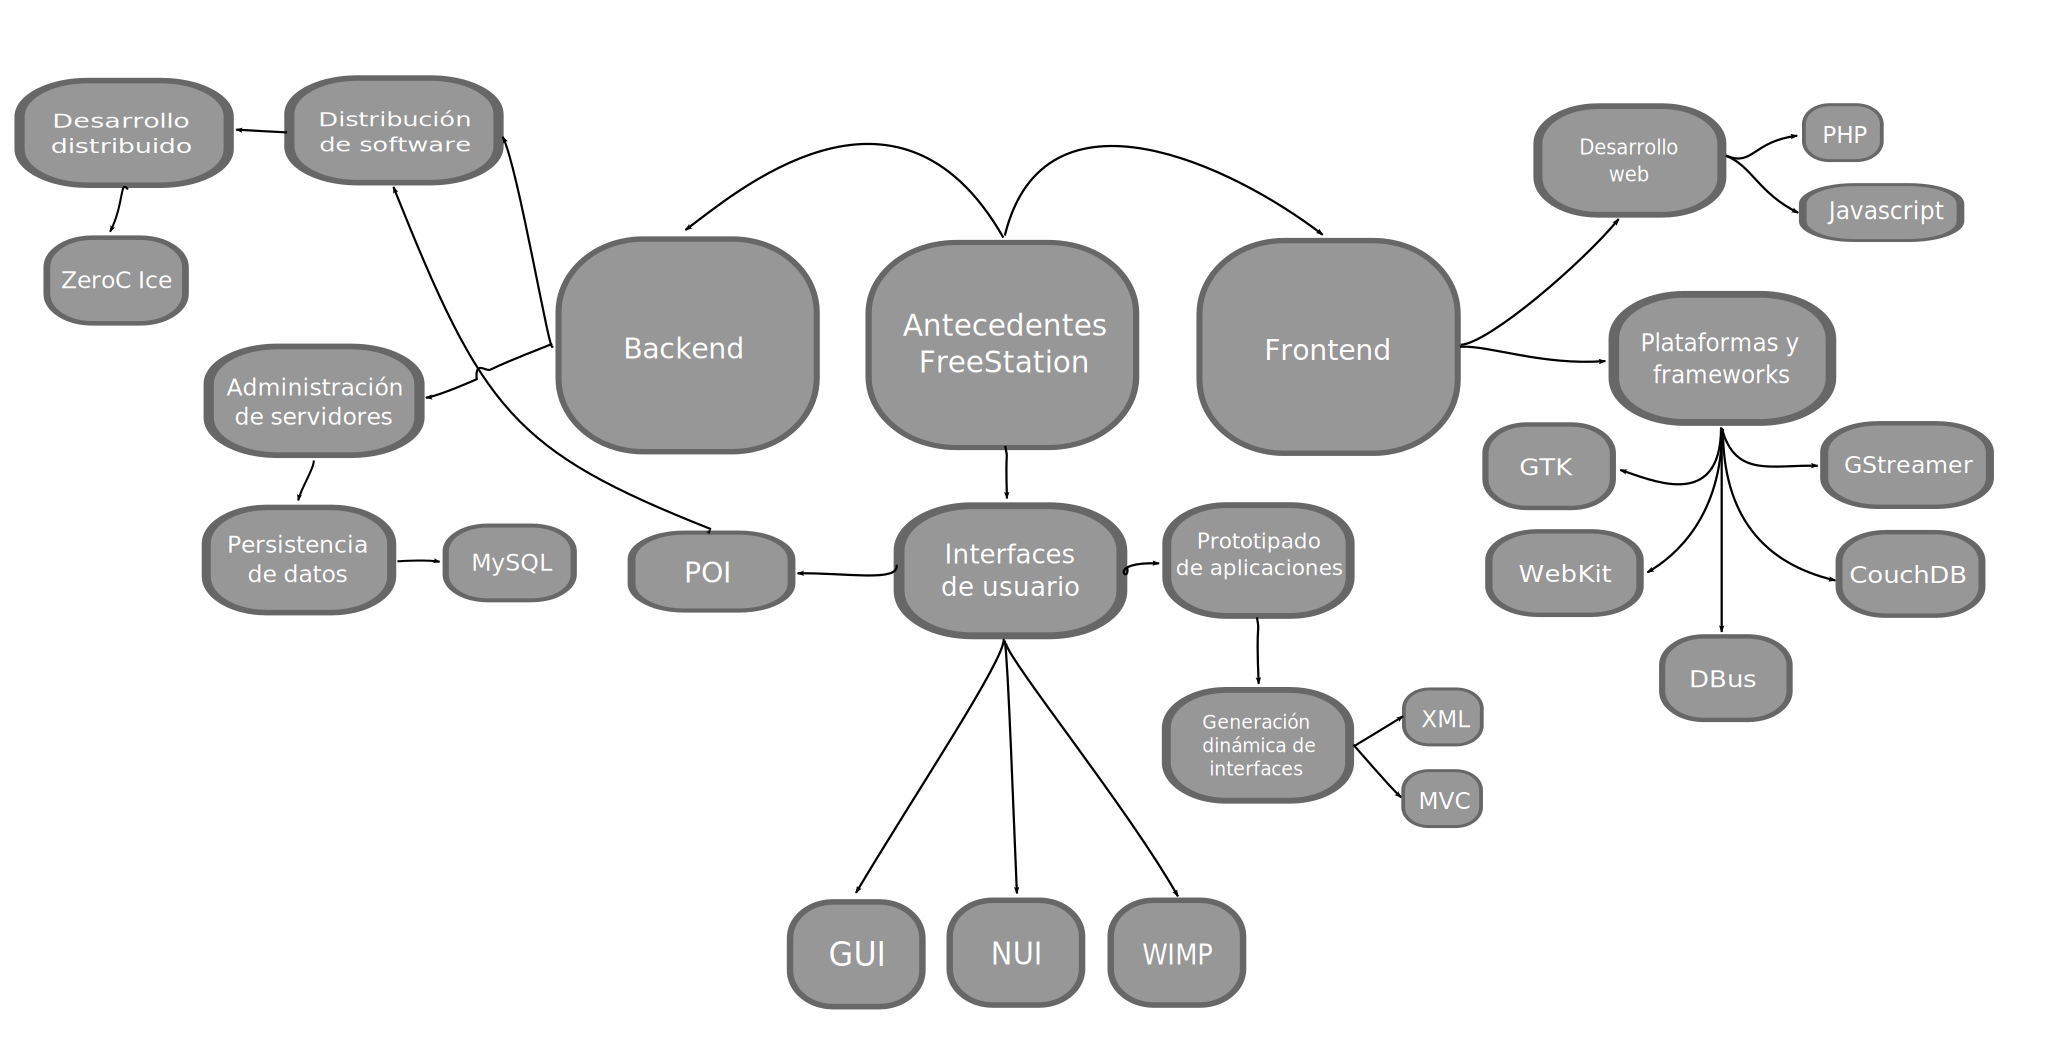
\includegraphics[width=450px]{src/img/conceptual-map-vectorized.pdf}
        \caption[Mapa conceptual] {Mapa conceptual}
        \label{fig:MapaConceptual}
    \end{center}
\end{figure}

En la Figura ~\ref{fig:MapaConceptual} se muestra un mapa conceptual de los
contenidos descritos en este capítulo. Los antecedentes del proyecto se
describen en base al \emph{Frontend} del proyecto (necesario para la realización
de componentes que integran la parte visual mostrada al usuario) y el
\emph{Backend} (necesario para llevar a cabo las tareas internas para los
mecanismos implicados en la base de la aplicación). 

\newpage
La parte \emph{Frontend} se basa en el desarrollo web (principalmente PHP y Javascript)
y el uso de plataformas y frameworks como GTK, WebKit, DBus, Gstreamer o
CouchDB.

Por otro lado, el \emph{Backend} sirve al propósito de la distribución de software,
aplicando métodos de programación distribuida que están basados en tecnologías
de la biblioteca ZeroC Ice. Para ello se necesita de conocimientos de administración de
servidores, en particular gestión de persistencia de datos (basada en MySQL).

A su vez el proyecto necesita de una
base de interfaces de usuario, estudiando los diferentes enfoques de composición
de aplicaciones \acs{GUI}, \acs{NUI}, \acs{WIMP} y su utilización en 
\acs{POI}. De esta forma se requiere del estudio de mecanismo para el
prototipado de aplicaciones.
Es posible aplicar dicho concepto a través de la generación dinámica de interfaces que tienen como pilares la composición en formatos \acs{XML} y
patrones de diseño \acs{MVC}. 

Dentro del desarrollo e investigación actual, la elaboración del marco de
trabajo consiste en canales de distribución software generales\cite{Lan10}, con
personalización sencilla para usuarios poco avanzados. Dichos
medios de difusión, suelen requerir mucho esfuerzo a sus administradores y no
cuentan con fáciles interfaces de administración. Pese al creciente acceso a
conexiones de alta velocidad en el ámbito doméstico, los usuarios no disponen
de un mecanismo cómodo de acceso a software e información directamente asociado
a su perfil en una determinada organización.

Es pues, un tema abordado heurísticamente, pero con soluciones poco prácticas y
elaboradas que requieren de una mejora constante
atendiendo a las necesidades del usuario final.

En este capítulo se estudian algunas de las principales áreas en las que se basa
el presente Proyecto Fin de Carrera. Estos contenidos serán citados en capítulos
posteriores, por servir de base teórica para el diseño y desarrollo de
FreeStation.

\newpage

\section{\uppercase{Introducción}}

La simplicidad de un componente de acceso público facilita a comunidades de
clientes la manera de obtener datos, informes o documentación de uso público.

Los residentes locales pueden ver más factible encontrar la información que
necesitan en un momento preciso si ésta se encuentra orientada en el 
contexto de su situación actual. Esto puede ahorrar tiempo y costes, en lugar
de realizar a una llamada a una operadora de información.

Éste el punto fuerte de los kioscos: ofrecer un mayor nivel de información sin
requerir una gran infraestructura. De este modo es posible ahorrar en recursos 
manteniendo el nivel de calidad al usuario final. 
En los kioscos informativos, la información es actualizada al momento y no está
sujeta a errores y confusiones entre operadores intermediarios.

El origen de los kioscos proviene de Persia. Los otomanos adoptaron el
concepto a través de los sultanes. Estos lo usaban en sus residencias locales
para disponer de un mercado cercano, sin gastar gran cantidad de tiempo en
viajes extraordinarios. El concepto también fue exportado a Europa para venta de
cigarrillos, flores o artículos exóticos. La gran ventaja era la variedad
ofrecida en un pequeño punto en particular y cercano. Los kioscos multimedia
siguen un propósito parecido en un ordenador.

Los kioskos son un gran mercado en auge. La empresa Griffin Chase Oliver lleva
produciendo kioscos desde 1978. Su tasa actual de fabricación son 150 
unidades por mes.\footnote{Griffin Chase Oliver:\\
\url{http://www.griffinchaseoliver.com/Library/downloads/how_to_budget_pop_displays.pdf}\label{ftn:Griffin}}

Otras empresas interacciones como Four Winds Interactive (FWi) poseen el ranking
de empresa número 660 en 2011 de las 500 empresas más importantes en Estados
Unidos. Es una de las compañias de América que más rápido han crecido en los
últimos 3 años. Los puestos directos e indirectos se estiman en 350.000 con unos
beneficios de 366 millones de dolares en el año 2011\footnote{Four Winds
Interactive:\\
\url{http://www.fourwindsinteractive.com/press/pr-2011-inc-5000.htm}\label{ftn:Griffin}}. FWi ha basado su negocio
en desarrollar más de 65.000 kioskos digitales para hospitales, centros
educativos y otros.

\section{\uppercase{POI y proceso de distribución}}
\label{sec:distributionaccesspoi}

Los terminales de tipo «Puntos de interés» (Point Of Interest \acs{POI}) han
avanzado significativamente con la tecnología de los últimos años, habilitando 
su integración en casi cualquier lugar con un uso sencillo (la empresa Griffin
Chase Oliver creó desde 1990 POI analógicos para bancos).

Esta tecnología integrada ha permitido la interacción en edificios con sus
visitantes. En determinadas instituciones como colegios, institutos,
universidades, ayuntamientos u oficinas de turismo es común ver pequeños 
puntos donde se
encuentran terminales mostrando información a los transeúntes. Algunos
terminales incorporan mecanismos de interacción mediante teclado, ratón o
incluso de forma táctil, pero estos paradigmas pueden ser mucho más complejos

En la panorámica del proceso de distribución de información, o más concretamente
del proceso de distribución software, la tendencia actual marca la utilización
de las redes de comunicación\cite{Ver02}.
La potencia actual de las mismas permite satisfacer las necesidades de
información de los usuarios en base a arquitecturas específicas adaptadas a la
constante evolución de los contenidos.~\\

\begin{figure}[ht]
    \begin{center}
        \includegraphics[width=425px]{src/img/front-poi-dni-combined.jpg}
        \caption[POI de la Policía para DNIe]{POI de la Policía para DNIe}
        \label{fig:POIDNI}
    \end{center}
\end{figure}

Los últimos servicios de la administración se mueven y avanzan en la dirección
de incorporar las últimas tecnologías al alcance del usuario regular. Este
avance requiere de especificaciones concretas y herramientas que permitan
automatizar los procesos involucrados. Varios de estos servicios se han 
empezado a ofrecer al público de forma experimental en ciertos entornos de
explotación específicos.

Uno de estos grandes hitos ha sido la incorporación del DNI electrónico (DNIe) y
sus consecuentes POI para facilitar trámites burocráticos (pago de multas,
renovación de datos, solicitud de certificados, etc).

En la imagen de la figura ~\ref{fig:POIDNI} se observa un POI en una comisaría
de policía. Dispone de un teclado, trackball y un lector de DNI electrónicos.

\begin{figure}[ht]
    \begin{center}
        \includegraphics[width=425px]{src/img/adif-sescam-combined.jpg}
        \caption[POIs de la estación de trenes ADIF (a), Sescam (b) y
        (c)] {POIs de la estación de trenes ADIF (a), Sescam (b) y
        (c)}
        \label{fig:POI_ADIF}
    \end{center}
\end{figure}

Es interesante recalcar que cuenta con un cable de conexión a internet para descarga de
información. El punto de interés se encuentra ubicado en la entrada a la
comisaría. La entrada está cubierta para evitar daños ambientales por lluvia u otros
elementos, pero es accesible al público en cualquier momento del día o
de la noche.

\newpage 
La vigilancia del POI está permanentemente asegurada por cámaras las 24 
horas y de forma presencial durante el horario diurno.

Como se puede apreciar en la imagen de la figura ~\ref{fig:POIDNI}, la pantalla
muestra con más detalle campos de entrada para el usuario y una simple 
interfaz accesible con botones.
La altura del POI esta ajustada para gente discapacitada en silla de ruedas e
incorpora síntesis de voz para personas ciegas.

En la imagen de la figura ~\ref{fig:POI_ADIF} se corresponde a un POI en una
estación de trenes Adif. El diseño es totalmente diferente a los analizados 
con anterioridad.
Muestra una gran pantalla en vertical y rotada. Es posible que disponga de
funcionalidad táctil y conexión a internet.

Es remarcable la incorporación de un sistema de audio para persona ciegas y
como posible utilización de confirmación para notificaciones de audio. Por sus
características no parece ser muy adecuada para personas en sillas de ruedas,
por lo que su funcionalidad puede estar limitada a un panel de información de
baja interacción.

La imagen de la figura ~\ref{fig:POI_ADIF} (b) es otro ejemplo de POI
interesante y bastante diferente ya que dispone de un teléfono o intercomunicador para 
asistencia directa, teclado, trackball, ratón y lector
de tarjetas sanitarias. Existe una bandeja impresora para enviar datos
útiles impresos como informes al usuario. En la imagen de la figura
~\ref{fig:POI_ADIF} (c) puede apreciarse con mayor detalle la funcionalidad del
punto de interés.

Este es un conjunto reducido de ejemplos de la gran variedad de POIs.
Normalmente varias unidades similares se pueden encontrar en los mismos centros,
universidades, estaciones de policía, hospitales, etc. El modelo de
administración actual de los POIs causan que sea difícil su mantenimiento. Es
muy habitual que, con el tiempo, cada unidad de POI presente averías, fallos
software, inconsistencias.

De este modo, es necesario disponer de una plataforma para gestionar y
solucionar, en la medida de los posible, este tipo de problemas. El sistema de
gestión debe ser capaz de poner en producción y configurar POIs con diversas
versiones de software, notificaciones de estado, así como reinicio automático en
caso de fallo grave, FreeStation trata de cubrir estas necesidades en gestión y
mantenimiento de POIs heterogéneos.

\subsection{\uppercase{Guías de diseño en POI}}
\label{sec:guiadesignpoi}

Como casos de estudio de gran éxito en el desarrollo de POIs pueden citarse el
Sistema de Información de la Expo'92 de Sevilla\cite{Mag07} y el Sistema de
Mensajes de los Juegos Olímpicos de 1984\cite{GoB87}.

Los sistemas POI son diseñados para ser usados en
modo ``\emph{walk up and use}'', es decir, para caminar y usar. Ello hace
mención a que los sistemas POI deberían ser tan autoexplicatorios como fuera 
posible. Los usuarios tienen poco tiempo para usar el sistema, por ello el
sistema debe ser capaz de producir la información necesaria de forma rápida. Si un usuario
queda atascado en la interacción, se frustrará y no volverá a usarlo.

Dichos sistemas, también deben detectar si el proceso de interacción queda
abandonado y volver al estado inicial si no hay nuevas acciones. El
temporizado para volver al estado inicial, no debería ser pequeño, para evitar
frustraciones para usuarios que necesitan de un mayor tiempo para llevar a cabo
sus acciones (como lectura extensa de textos).

En esta sección hemos estudiado la distribución de POIs y su evolución. En la
siguiente sección se explicará la caracterización de funcionalidades posibles.

\section{\uppercase{Caracterización de los POIs}}

Aparte de las guías de diseño, un POI puede estar caracterizado según las
funcionalidades que estén presentes para el usuario. A continuación se describen
algunas:

\begin{itemize}
  \item{\textbf{Entrada de datos por voz}\\
  La entrada datos por voz incrementa la fiabilidad de uso del
usuario\cite{Mag07}, independientemente de la confiabilidad del sistema de
reconocimiento por voz.

En un POI pueden incorporarse teléfonos, auriculares, micrófonos u otros
dispositivos que permitan mejorar la interacción del usuario y faciliten el uso
a personas que no dispongan de las habilidades necesarias. El principal problema
es la distinción de palabras clave para el sistema. Este campo ha 
avanzando significativamente en los últimos años, pero la tasa de error
todavía es considerablemente alta. 

\newpage
Estos métodos implican también la pérdida
de privacidad y contaminación de ruido en un entorno abierto al tener que producir
verbalmente los datos.

A pesar de esas limitaciones, los beneficios aportados por la entrada de
datos por voz son más significativos que la entrada de datos estándar de texto
mediante teclados.
  }
  \item{\textbf{Música ambiente y sonidos de salida}\\
  La música en un POI puede ofrecer información extra\cite{Mag07} para
  presentación multimedia. Puede complementar a textos, iconos e imágenes para
impactar al usuario en mayor grado.

Es importante que usuario no perciba como intruso la incorporación de un sonido
ambiente o incluso distraiga del contenido principal. Los sonidos cortos y
agudos provocarán rechazo en el usuario al igual que bucles intermitentes muy
cortos de sonido ambiente.
  }
  \item{\textbf{Estructura y navegación}\\
  La estructura debe ser simple\cite{LoM99} para que el usuario se sienta cómodo
  en la interacción. El sistema debe tener un punto de entrada al que el usuario debe
poder volver en cualquier momento que desee. Normalmente a este punto inicial se
le denomina Pantalla de bienvenida o menú principal.

El resto de contenido idealmente debe estar estructurado en pantallas
seleccionables desde esta etapa. Es recomendable si existe una jerarquía de
contenidos presentar una secuencia del camino recorrido. Esto conseguirá un
mejor posicionamiento conceptual de los contenidos.

Cada pantalla debe ser fácilmente distinguible de otras secciones y representar
acorde a sus contenidos la información. Se puede proporcionar un menú básico de
controles como \emph{Inicio/Fin/Atrás/Siguiente/Cancelar/Salir} que ayude al
usuario a tomar el control en sus acciones. En puntos críticos debería mostrarse una
doble confirmación al usuario mediante menús emergentes o reiteración de 
la acción.
  } 
  \item{\textbf{Personalización}\\
  La personalización en la interfaz debe permitir adaptar la capa de
  representación de la información a los gustos de cada grupo de usuarios.

Posibilitar configuraciones al usuario permite una mayor
integración\cite{Fis00}, pero complica el desarrollo. Algunas características
como los tamaños de las fuentes tipográficas, color o fondo suelen ser
fácilmente adaptables ofreciendo así mecanismos básicos de personalización de
interfaz.}
  \item{\textbf{Prueba de POIs en producción}\\
  \label{sec:poiproduccion}
Como sistema expuesto al público general un POI debería ser probado siguiendo
una serie de factores determinantes.

En un entorno real, los sujetos tendrán una experiencia previa o serán
totalmente ajenos al servicio. Los usuarios sin experiencia tienden a producir
problemas desconocidos y probar más profundamente el sistema.

Si existe la posibilidad, se deberían incluir usuarios con ciertos
perfiles desabilitados para algunas funciones o con funcionalidad reducida y
observar su comportamiento.
Esto facilitará probar partes del sistema por separado y centrarse en problemas
específicos.

En pruebas de carga del sistema, el rendimiento será crítico y aparecerán
errores desconocidos. Un sistema eficaz debería conocer sus límites máximos de
forma precisa\cite{Mag07}.
  } 
  \item{\textbf{Selección de idiomas}\\
  \label{sec:selectlanguage}
En una comunidad local puede ser necesario habilitar varios idiomas dependiendo
de la funcionalidad del POI. Un POI orientado a turismo idealmente debería
tener un número elevado de idiomas disponibles. 

El esfuerzo adicional de incorporar un idioma a menudo no es compensable al
número de usuarios que pueden utilizarlo, pero evita restringir la cuota de
acceso a dicho idioma. La alternativa más común es habilitar un conjunto de
iconos por idioma o banderas por territorio\cite{Mag07}. Si no es posible, 
una lista despegable con las opciones de idiomas o una pantalla dedicada al
cambio de idioma.

En general las opciones utilizadas con simbología o iconos son más rápidamente
accesibles para uso de otro idioma, ya que una lista de texto confunde al
usuario y retrasa su tiempo de percepción en el cambio de idioma. En el proceso,
el usuario debe ser capaz de realizar el cambio de idioma sin necesidad de 
hablar un idioma complementario.
  }
  \item{\textbf{Posicionamiento físico y localización}\\
En un comienzo la localización de un POI debe ser anunciada por
el servicio del centro. Esto permite dar conocimiento exacto a sus usuarios.
Elementos como indicadores en revistas, notas en puertas o ventanas adyacentes
pueden ayudar al usuario.

Se recomiendan indicadores de alto contraste en blanco/amarillo con caracteres
en fondo negro\cite{Mag07} para usuarios con visión reducida. También existe la 
posibilidad de proporcionar tarjetas que emitan un sonido audible hacia la 
localización del POI.

La manera más efectiva de que los usuarios encuentren el POI es situándolo en el
flujo normal del recorrido de usuario, por ejemplo en la entrada del edificio o
en el patio central de reuniones. Un POI de tickets de tren,
debería ser posicionado a la entrada de la estación y no en su final, para
facilitar la compra de los usuarios antes de entrar al tren.

Fomentar el uso de un POI por usuarios desarrolladores puede ser una buena
manera de involucrar a más personal en el mismo. Facilitar previamente POIs con
demostraciones de ejemplo y obtener retroalimentación de los usuarios 
casuales, permite disponer de un
criterio formado sobre su uso y la experiencia de visualización.

Según el objetivo de uso, pueden desarrollarse distintas formas de presentar el
contenido para rangos de edad de usuarios. Por ejemplo, es muy posible que
personas con edad más avanzada prefieran botones mayores con colores simples y
pocas animaciones.
  }
  \item{\textbf{Privacidad}\\
Los usuarios que utilizen un POI público pueden ser observados de cerca por
otros usuarios. El nivel de privacidad depende de los datos a visualizar.

Por ejemplo, la privacidad para consultar en un POI de turismo, suele ser baja
ya que no se requieren datos personales concretos. Sin embargo, en POIs donde
por ejemplo se necesiten introducir datos privados como un DNI para consultas
jurídicas puede ser necesario un alto grado de privacidad. 

En el desarrollo de POIs públicos se recomienda requerir la mínima información 
posible por parte del usuario. En el caso de necesitar estrictamente datos
confidenciales, el POI público debería de ser cerrado en una cabina donde
facilitar la privacidad de la entrada de datos del usuario. Estas medidas
evitarán el rechazo por parte del usuario a introducir datos.

Si se opta por esta última opción, para personas con discapacidad motriz
debería proporcionarse un acceso conveniente.
  } 
  \item{\textbf{Sencillez en menús}\\
Proveer menús de entrada sencillos para el usuario. Deben tener una redacción
concisa y clara para que el usuario tenga plena conciencia de la acción a
realizar. Adicionalmente los textos adicionales como leyenda pueden enriquecer
la acción. Según Ben Shneiderman el número máximo de elementos a
recordar en un menú por una persona tiende entre 3 y 7 de promedio\cite{Shn09}.
Un número más elevado resultará en una interfaz sobrecargada y de uso
complicado.
La estructura de las listas de menús debe estar cuidadosamente estudiada. Es
conveniente seguir algún orden de posicionamiento, bien por relevancia o
simplemente orden alfabético (por ejemplo Buscar, Imprimir, Mostrar, Salir)
Es importante recalcar espacios entre opciones para ayudar a enfatizar la
estructura.
Si existen listas de menú numeradas, se deben evitar los huecos en la secuencia
normal. Por ejemplo, del 1 al 9, no sería acorde saltar la opción 5, en su lugar
renombrar del 1 al 8.
De igual modo, sería conveniente evitar abreviaciones en opciones de menú que
sean poco conocidas al público, etc.
  } 
\end{itemize}

\subsection{\uppercase{Componente social}}

Combinando el componente social\cite{WaF94} de un objeto que se encuentra en el
exterior con la inmensidad de contenidos que pueden ofrecer una red
tecnológica es posible realizar una distribución de contenidos uniforme
orientada a docencia, turismo o cualquier sector que requiera de un
despliegue de contenidos.

Un objeto accesible en exteriores fomenta la participación del entorno.
Inicialmente despierta una gran curiosidad y una rápida propagación si ofrece
contenidos o información de utilidad para sus usuarios. Su practicidad queda
demostrada en casos de consultas urgentes, donde no existan persona físicas 
que puedan facilitar la información o en horarios no laborales.

\subsection{\uppercase{Beneficios y problemas jurídicos}}

La distribución de software conlleva una
responsabilidad asociada al marco de la legalidad. Cualquier software 
dispone de una licencia que habilita una serie de acciones permitidas, 
como es la distribución. En lo particular,
pueden surgir problemas jurídicos derivados si un POI no cuenta con la
debida autorización. Luego, estableciendo una determinada base tecnológica
con tendencia en la distribución de software libre, los problemas
legales en este aspecto suelen ser nulas o muy reducidas.

Por otro lado, la distribución de software beneficia al usuario final
ya que la compra individual supone requerir o disponer de unos costes
asumibles por cada software particular. La elección
entre un gran catálogo de software ahorra tiempo al usuario en la
búsqueda y obtención del mismo.

Este enfoque añade una serie de ventajas asociadas, como la alta
disponibilidad de nuevas versiones y actualizaciones de seguridad.
En el caso del Software Libre, estas características de alta
disponibilidad pueden traducirse igualmente en la personalización
de distribuciones para diversos colectivos de usuarios. 

\newpage

Estos paquetes de contenido específicos (formados por software,
documentación y ficheros multimedia) pueden ser adaptados a
necesidades concretas (docentes, de investigación o profesionales),
ahorrando gran cantidad de costes (temporales y económicos).

Por lo tanto, en un ecosistema basado en aplicaciones de software libre
que basa su distribución en estándares abiertos sin prácticamente
restricciones, la participación y progreso es elevado.
La practicidad de licencias como \acs{GPL}\label{acro:GPL},
\acs{LGPL}\label{acro:LGPL}, \acs{BSD}\label{acro:BSD},
\acs{MIT}\label{acro:MIT}, etc, permite usar el software libremente, copiarlo,
publicarlo, distribuirlo, siempre que se incluya la nota de copyright en todas las distribuciones.

\subsection{\uppercase{Estudio de mercado}}
\label{sec:marketstudy}

El entorno en el que se desenvuelve este PFC es el ámbito empresarial y de
organizaciones que necesitan comunicar y dotar a su público de puntos de
interés orquestándolos de una manera cómoda y sencilla.~\\

\begin{figure}[ht]
    \begin{center}
        \includegraphics[width=460px]{src/img/redhat-financial-perfomance.jpg}
        \caption[Rendimiento financiero RedHat 2007-2009] {Rendimiento financiero RedHat 2007-2009}
        \label{fig:Redhatrevenues}
    \end{center}
\end{figure}

\newpage

La necesidad y demanda de un mercado creciente en el sector del software
libre\cite{Asl09} garantiza la necesidad y aplicación de POIs en el futuro.
La industria se está expandiendo más rápidamente a nivel mundial debido a 
las crecientes necesidades de los mercados emergentes.
La reducción de costes y aumento de beneficios gracias al software libre es
un hecho para los sectores educativos y empresariales.

Los beneficios de empresas basadas en software libre como RedHat han mostrado un
crecimiento alcista desde su creación, alcanzado cifras de un billón de
dolares americanos en 2012\cite{McM12}. En el gráfico de la figura
~\ref{fig:Redhatrevenues} se observa el gran crecimiento financiero para RedHat.

\begin{figure}[ht]
    \begin{center}
        \includegraphics[width=460px]{src/img/ubuntu-market-share.png}
        \caption[Tasa de mercado de
        distribuciones GNU/Linux] {Cuota de mercado de
        distribuciones GNU/Linux}
        \label{fig:ubuntumarketshare}
    \end{center}
\end{figure}

Otro caso de éxito es Ubuntu, perteneciente a la empresa Canonical. Como muestra
la figura ~\ref{fig:ubuntumarketshare} las estadísticas web sugieren que el
porcentaje de mercado de Ubuntu dentro de distribuciones GNU/Linux es de
aproximadamente un 49\%\footnote{StatOwl :Operating System Version Market Share:\\
\url{http://statowl.com/operating_system_market_share_by_os_version.php?1=1&timeframe=last_6&interval=month&chart_id=4&fltr_br=&fltr_os=&fltr_se=&fltr_cn=&limit[]=linux}
\label{ftn:ubuntumarketshare}}, y con una tendencia a subir como servidor
web. 

En los últimos años las instituciones públicas poco a poco han realizados
migraciones importantes hacia el software libre.
Islandia aprobó un decreto en 2008 que se aplica contundentemente para la
totalidad de las instituciones públicas.\footnote{Free and Open-source Software
- Government Policy of Iceland:\\
\url{http://eng.forsaetisraduneyti.is/information-society/English/nr/2882}
\label{ftn:ubuntuislandia}}

\newpage

En 2007, el Ministerio de Educación y Ciencia de la República de Macedonia
desplegó más de 180.000 equipos de escritorio con Ubuntu preinstalado para 
su uso en las aulas, y animó a cada estudiante del país a usar 
computadoras con Ubuntu.\footnote{Every Student in the Republic of Macedonia to Use Ubuntu-Powered Computer
Workstations:\\
\url{http://www.ubuntu.com/news/macedonia-school-computers}
\label{ftn:ubuntumacedonia}}

La policía francesa, desde 2009, está en proceso de instalar Ubuntu en 90.000
estaciones de trabajo, demostrando un 70\% de ahorro en el presupuesto de TI sin
tener que reducir su capacidad.\footnote{French police: we saved millions of euros by adopting Ubuntu:\\
\url{http://arstechnica.com/information-technology/2009/03/french-police-\\saves-millions-of-euros-by-adopting-ubuntu/}
\url{http://www.canonical.com/sites/default/files/active/Casestudy-GendarmerieNationale.pdf}
\label{ftn:ubuntufrenchpolice}}. En 2011 tuvo un importante incremento activo
de 20 millones de usuarios\footnote{Retail Stores in China:\\
\url{http://blog.canonical.com/2011/10/27/retail-stores-in-china/}
\label{ftn:ubuntum20million}}. 

La demanda de necesidad es creciente en el 
ámbito empresarial y las administraciones públicas. Aproximadamente el
39\%\footnote{CENATIC: El Software Libre en el Sector Español de Servicios
Informáticos\\
\url{http://observatorio.cenatic.es/index.php?option=com_content&view=
article&id=741:el-software-libre-en-el-sector-espanol-de-servicios-informaticos&catid=13:empresas&Itemid=23}
\label{ftn:ubuntustatsspain}} de
empresas de España afirman haber comercializado productos bajo una licencia 
de software libre o fuentes abiertas o haber realizado actividades 
relacionadas con dicha tecnología. 

La cifra de negocio estimada derivada de la
venta de productos de software de fuentes abiertas alcanzó en 2010 los 
776 millones de euros. Esta cifra representa el 3,36\% del total del sector de
Servicios Informáticos y dio trabajo a cerca de 40.000 personas que estuvieron
implicadas en proyectos de consultoría o desarrollo de software de fuentes 
abiertas.

La formación también es un aspecto clave en el negocio del software libre.
Aproximadamente la mitad de las empresas (52\%) han proporcionado a sus
empleados formación sobre software de fuentes abiertas.

La tendencia en general es que la mayor parte de las empresas que en la
actualidad comercializan productos o servicios basados en software de 
fuentes abiertas, el 86\%, afirman que en el medio plazo, de aquí a 5 años,
seguirán comercializando este tipo de tecnología. 

\newpage

Entre las empresas que actualmente no comercializan soluciones libres, una de 
cada cinco empresas tiene previsto empezar a trabajar con este software con el
fin de poder ofrecérselo a sus clientes. Casos de éxito como en Andalucía, donde
se instalaron 220.000 equipos con Ubuntu \footnote{Andalusia deploys 220,000 Ubuntu desktops in schools throughout the region:\\
\url{http://www.canonical.com/about-canonical/resources/case-studies/andalusia-deploys-220000-ubuntu-desktops-schools-throughout-r}
\label{ftn:ubuntumandalucia}}. El software Lliurex (derivado de Ubuntu) permite
ahorrar 30 millones a la Generalitat desde 2005\footnote{CENATIC: El software
Lliurex permite ahorrar 30 millones a la Generalitat desde 2005:\\
\url{http://www.cenatic.es/hemeroteca-de-cenatic/3-sobre-el-sector-del-sfa/40024-el-software-lliurex-permite-ahorrar-30-millones-a-la-generalitat-desde-2005}
\label{ftn:ubuntuliurex}}

Las empresas de software libre tienen un mayor crecimiento en sectores
empresariales, servidores o en educación donde se exploran formas
interactivas para dotar a los alumnos de mayores facilidades. 

\begin{figure}[ht]
    \begin{center}
        \includegraphics[scale=0.8]{src/img/linux-jobgraph.png}
        \caption[Gráfico de tendencias de trabajo para Windows, Linux, Mac
        2006-2012] {Gráfico de tendencias de trabajo para Windows, Linux, Mac
        2006-2012}
        %% http://investors.redhat.com/financials-statements.cfm
        \label{fig:jobs}
    \end{center}
\end{figure}

Asimismo, un ecosistema de aplicaciones derivadas puede surgir como forma de
personalizaciones y adaptaciones al software original, lo que garantiza un buen
mercado de explotación para los desarrolladores. En la gráfica de la figura
~\ref{fig:jobs} se puede observar una comparación entre los trabajos más
demandados para diferentes plataformas. Según \cite{Ind12} en los últimos años
la mayor demanda de trabajo ha sido experimentada para la plataforma GNU/Linux.

En esta sección hemos estudiado el mercado relativo al software libre. Uno de
los objetivos de FreeStation es facilitar su distribución en POIs, que cuentan
con elevados requisitos relativos a la facilidad de uso y a los mecanismo de
interacción. En la siguiente sección estudiaremos los principios de diseño de
interfaces naturales.

\section{\uppercase{El diseño de interfaces naturales}}
\label{sec:interfazNUI}
Una interfaz es el medio de comunicación entre un usuario y un ordenador.
Requiere de un lenguaje preciso para comunicar al usuario con el
ordenador. La construcción de una interfaz de usuario natural o
\acs{NUI}\label{acro:NUI} sigue unas líneas guía de diseño específicas. El
término natural mimetiza con el significado de "mundo real". Es un proceso
iterativo que crea un producto asumiendo que el usuario debe sentirse 
libre. Una interfaz debe hacer que usuario actúe de forma natural y que esta
se sienta natural. La utilización de interfaces naturales a través de un diseño
riguroso y aprovechamiento potencial de tecnologías modernas permiten una utilización con
mayor similitud a las habilidades humanas.

Un ejemplo de ello, son las interfaces de usuario desarrolladas en un ambiente
de dispositivos multitáctiles o \emph{multi-touch} que mantienen una entrada de 
usuario muy adecuada a una forma natural de interacción.
Comparándolo con las interfaces desarrolladas para ratón, permiten la
implementación de nuevos paradigmas de interacción, potenciando la expresividad
de las acciones del usuario. Al contrario que las interfaces
\acs{WIMP}\label{acro:WIMP} diseñadas para una interacción basadas en ratón, las interfaces \emph{multi-touch} aprovechan mejor
el concepto de memoria espacial del usuario y tienen una gran aceptación en la
información que realmente llega a percibir el usuario en su uso.

\begin{figure}[ht]
    \begin{center}
        \includegraphics[width=300px]{src/img/check-buttons-state1.png}
        \caption[Ejemplo 1 interacción con interfaz NUI]
        {Selección NUI de una caja de comprobación: (1) Estado inicial con los elementos
        desactivados (2) Interacción del usuario con un gesto
        natural para selección horizonal (3) Resultado con caja de
        comprobación seleccionada.}
        \label{fig:NUI1}
    \end{center}
\end{figure}

\newpage

Las interfaces NUI aprovechan el contexto como principio fundamental de diseño,
empleando mecanismos de sincronismo y favoreciendo la componente social de la
interacción (colaboración múltiple).

\begin{figure}[ht]
    \begin{center}
        \includegraphics[width=300px]{src/img/check-buttons-state2.png}
        \caption[Ejemplo 2 interacción con interfaz NUI]
        {Selección NUI de múltiples cajas de comprobación: (1) Estado inicial
        con los elementos desactivados (2) Interacción del usuario con un gesto
        natural para selección vertical (3) Resultado de todas las cajas de
        comprobación seleccionadas.}
        \label{fig:NUI2}
    \end{center}
\end{figure}

En las figuras ~\ref{fig:NUI1} y ~\ref{fig:NUI2} se muestran ejemplos ilustrados
de hipotéticas interacciones NUI donde el usuario tendría un beneficio de
interfaz adaptada a un uso más natural. La desventaja de utilizar una primitiva
de interacción como la selección cruzada es que puede existir un alto grado de
falsos positivos debido a una interacción descuidada por parte del 
usuario. Por ello, este nuevo paradigma permite el desarrollo de interfaces que
ofrezcan un comportamiento más cercano al que espera intuitivamente el usuario.

Por tanto, Las interfaces de usuario se deben elaborar,
investigar y someterse a un proceso de ingeniería como parte de una aplicación.
La mayoría de creadores de interfaces no analizan realmente una interfaz de
usuario, sino que se limitan a reaprovechar el diseño de otras interfaces
similares y adaptar de forma iterativa la interfaz a sus requisitos.

\subsection{\uppercase{La coexistencia de modelos de interfaces}}

Los conceptos de NUI y GUI probablemente coexistan prósperamente en el 
futuro. Por ejemplo, una NUI puede estar bien adaptada en un nicho de mercado
como el entretenimiento. Contribuye a destacar en la visualización de 
contenido, ejemplos interactivos, animaciones y juegos. Al mismo tiempo, el
contenido viene transferido desde el mundo GUI, donde se necesita para 
interacciones como acciones e integración de contenido.

Los elementos entre ambos son transferibles. Un botón de GUI de una aplicación
de escritorio, puede extrapolarse fácilmente para una pantalla de navegador en
un coche, adaptando la idea de interacción mediante dispostivo táctil o comando
de voz.

Pero esto no es cierto en la mayoría de ejemplos de NUI a GUI. Una interfaz NUI
que disponga de un diseño horizontal y vertical, no adapta bien al modelo
simultáneo en una GUI. Las interfaces NUI toman el fuerte principio de la acción
del usuario y adaptan la interfaz al uso tradicional.

\subsection{\uppercase{Menos es más}}

Iniciar un diseño simple es una oportunidad para construir interacciones simples
que ayuden a aplicar tareas complejas. En cada generación de interfaces, los
desarrolladores y diseñadores tratan con el desafío de construir 
aplicaciones para explotar las ventajas que ofrecen las
nuevas interfaces.

El riesgo de construir nuevas aplicaciones reside en reutilizar los principios
que fueron válidos y mayormente usados en las aplicaciones anteriores. Olvidar
los estilos de interacción antiguos es necesario para innovar en aplicaciones 
tradicionales. Sin embargo, debe tener el uso fundamental y asumido
por la experiencia de usuario anterior.

Las guías de diseño de interfaces NUI recomiendan:

\begin{itemize}
  \item Probar las mecánicas fundamentales de las interacciones primarias antes
  de reconstruir o desechar cualquier interacción. Si el usuario acepta los
  cambios de forma positiva, continuar el desarrollo con cambios leves en cada
  iteración.
  \item Estudiar el diseño de aplicaciones NUI existentes. En general, los
  usuarios se comportaran de forma similar para procesos NUI ya probados y
  aceptados.
  \item Restringir el dominio de mecánicas de interacción. Un buen enfoque para
  desarrollar una tarea compleja de interacción, es dividir la tarea en regiones
  y tratar cuidadosamente cada parte de diseño.
  \item La interacción debe ser divertida y recompensar al usuario
  con algún beneficio por su uso.
  \item El usuario debe focalizarse en el contenido. Por ejemplo la
  compartición de fotos, la exploración de configuraciones de
  productos, etc.
  \newpage
  \item Tener al contexto de la aplicación como ciudadano de primera clase. La
  simbiosis entre el entorno y el usuario conllevan varias implicaciones para el
  diseño y su evaluación.
\end{itemize}

\subsection{\uppercase{La interfaz derivada de usuario}}
\label{sec:interfazderivada}
\begin{quote}
All science is experiential; but all experience must be related back to and derives its
validity from the conditions and context of consciousness in which it arises, i.e., the
totality of our nature.
— Wilhelm Dilthey
\end{quote}

Traducido al español:

\begin{quote}
Toda la ciencia es experimental, pero toda la experiencia debe estar relacionada
con retroceder y deriva su validez de las condiciones y el contexto de la
conciencia en las que surge, es decir, la totalidad de nuestra naturaleza.
— Wilhelm Dilthey
\end{quote}

El enfoque correcto para crear una interfaz natural NUI debería ser basado en un
sistema democrático. Permitiría a los usuarios definirlo desde su origen. 

Un método para llevara a cabo este propósito puede ser ofrecer a los usuarios
varios estados finales de la aplicación y sus funcionalidades y permitir al
usuario elegir los más convenientes. Destilando las acciones por la mayoría de
usuarios debería resultar en una síntesis de opciones bastante correcta.

Al enfoque de crear una interfaz de usuario basada en el contexto proporcionado
por usuarios y sus acciones se denomina ``Interfaz derivada de usuario'' o del
inglés The User-Derived Interface (\acs{UDI}\label{acro:UDI})

El enfoque UDI ha sido bastante útil y exitoso para interfaces pequeñas y que no
requieren de entrenamiento. Por ejemplo para interfaces de comando por voz,
suelen ser útiles para conocer que palabras exactas demandan los usuarios para
realizar una acción (``Enviar un correo a Juan'')

\newpage

En un proceso iterativo el analizador incluiría sinónimos, desambiguación o
palabras similares con ligeros errores de pronunciación. En resumen, crear una
interfaz NUI requiere de mucha retroalimentación de usuarios, para elegir 
buenos métodos de desarrollo y evaluación.

Normalmente un método efectivo de evaluación es el conocido como \acs{RITE}\label{acro:RITE} (Rapid
Iterative Testing and Evaluation). Es un método diseñado para un desarrollo y
diseños rápidos. Anima a interactuar con el aprendizaje de nuevos paradigmas y
hacer esfuerzos en la maneja de pensar el diseño con retroalimentación perpetua.

En esta sección hemos estudiado el diseño de las interfaces naturales y como
sus principios afectan en los objetivos de Freestation para el desarrollo de
interfaces. En la siguiente sección estudiaremos la generación dinámica de
interfaces.

\section{\uppercase{Generación dinámica de interfaces}}
\label{sec:generacionint}
La inteligencia artificial trata de simular las capacidades humanas mediante
el uso de máquinas y algoritmos. La comunicación es un campo imprescindible para
la simulación de las capacidades humanas. Puede darse entre máquinas
y máquinas o bien entre máquinas y seres humanos. El el segundo caso, la materia
\acs{IPO}\label{acro:IPO} trata con el análisis, diseño, implementación y 
evaluación de la interfaz de usuario\cite{LoM99}.

La investigación de Ben Shneiderman\cite{Shn09} está relacionada en este campo y
ha contribuido con importantes conceptos como 
la ``Usabilidad Universal'' o las 8 reglas de oro \footnote{Las 8 reglas 
son: coherencia, usabilidad universal, retroalimentación, prevenir
errores, reversión de acciones de forma sencilla, control por el usuario,
carga cognitiva, diálogos resolubles.}
    \label{ftn:8rules} que regulan el diseño de
interfaces de usuario. 

Existe una enorme comunidad de investigadores dedicados al estudio de técnicas que 
mejoren la usabilidad\cite{Shn89}, ya que una buena gestión de la interacción
supone la utilización de forma eficiente de una aplicación.

La generación dinámica de interfaces surge de la necesidad de disponer de
un enfoque generalizado durante la etapa de diseño de una
aplicación\cite{Bar09}. Se entiende como ``generación dinámica de interfaz``
aquella que es creada en tiempo de ejecución.

\newpage

Normalmente, las interfaces son generadas a través de soluciones estáticas.
Estas son desarrolladas con unos requisitos base especificados que normalmente
no varían en modelos normales. La especificación de requisitos se convierte en
una de las partes de mayor relevancia para la obtención de software de calidad.

Debido a que son desarrollos a medida y muy específicos, se crea una situación
en la que se hace prácticamente imposible la reutilización de
interfaces\cite{Fis00}, al menos sin implicar un gran coste de desarrollo en tiempo y recursos para
adaptar las interfaces a las nuevas necesidades. Una interfaz de fácil
aprendizaje conlleva muchas iteraciones para refinar un resultado final.

Por lo tanto, el enfoque más lógico es evitar las dependencias particulares de las
interfaces y tratar de aislar lo máximo cada componente. Las interfaces gráficas
se generadas de forma dinámica se adaptan en la medida de lo posible a las
características de cada proyecto.

Esta abstracción se consigue normalmente a través de estructuras de datos
asociadas a metadatos (datos que describen otros datos). Los metadatos permiten
explicitar relaciones entre datos y visualización de los mismos.

Existen enfoques prácticos de desarrollo de interfaces de usuario basados en
modelos de esquemas XML\cite{IEE05} con fácil acceso mediante una jerarquía
\acs{DOM}\label{acro:DOM}\cite{W3C00}.

Por ejemplo, en\acs{GTK+}\label{acro:GTK+}, se utiliza un visor de interfaces
dinámicas llamado Glade, que permite generar una interfaz en XML\cite{ZaM06} y cargar los componentes de
forma dinámica y en tiempo de ejecución desde una aplicación.

De igual forma, las aplicaciones desarrolladas en el sistema operativo Android
de Google, permiten la generación de vistas de aplicación basadas en XML. Para
este tipo de enfoque, los pilares fundamentales deben ser definidos de forma 
muy concreta. De esta forma, una misma estructura puede utilizarse como
base para proyectos con requisitos muy similares o incluso convertirse en
un patrón específico para el desarrollo\cite{LoM99}.

\newpage

\begin{figure}[ht]
    \begin{center}
        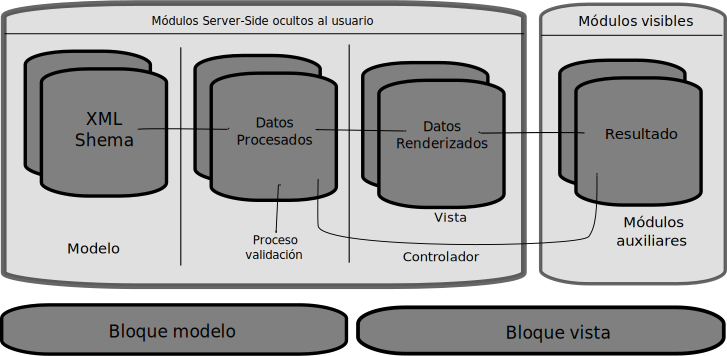
\includegraphics[width=460px]{src/img/diagrams/esquema-modulos-xml.pdf}
        \caption[Esquema de modelo-vista-controlador con XML] 
        {Esquema de modelo-vista-controlador con XML}
        \label{fig:esquemaXML}
    \end{center}
\end{figure}

La representación del modelo origen contiene los datos o
requisitos de la interfaz. Estos pueden incluir campos, tipos de datos y
multiplicidades, entre otros, que deben ser generados e incluidos en la interfaz
propuesta.

La aplicación debe ser capaz de comprender dichos
datos y generar de forma completa y correcta una interfaz. Incluso es posible
que la aplicación deba adaptarse de forma dinámica a cambios en el modelo de
entrada. Así el procesado de forma iterativa comtempla un comportamiento
adaptativo.

De esta forma la aplicación no es susceptible de ser dependiente de modelos
particulares y se evita por tanto una generación de interfaz estática o
invariable.

Generalmente este modelo y enfoque es utilizado en esquemas de 
Modelo-Vista-Controlador o \acs{MVC}\label{acro:MVC}. Es MVC es un patrón de
estructura para el diseño software, que constituye tres componentes para proporcionar
independencia con cada uno de ellos.

\newpage

\begin{figure}[ht]
    \begin{center}
        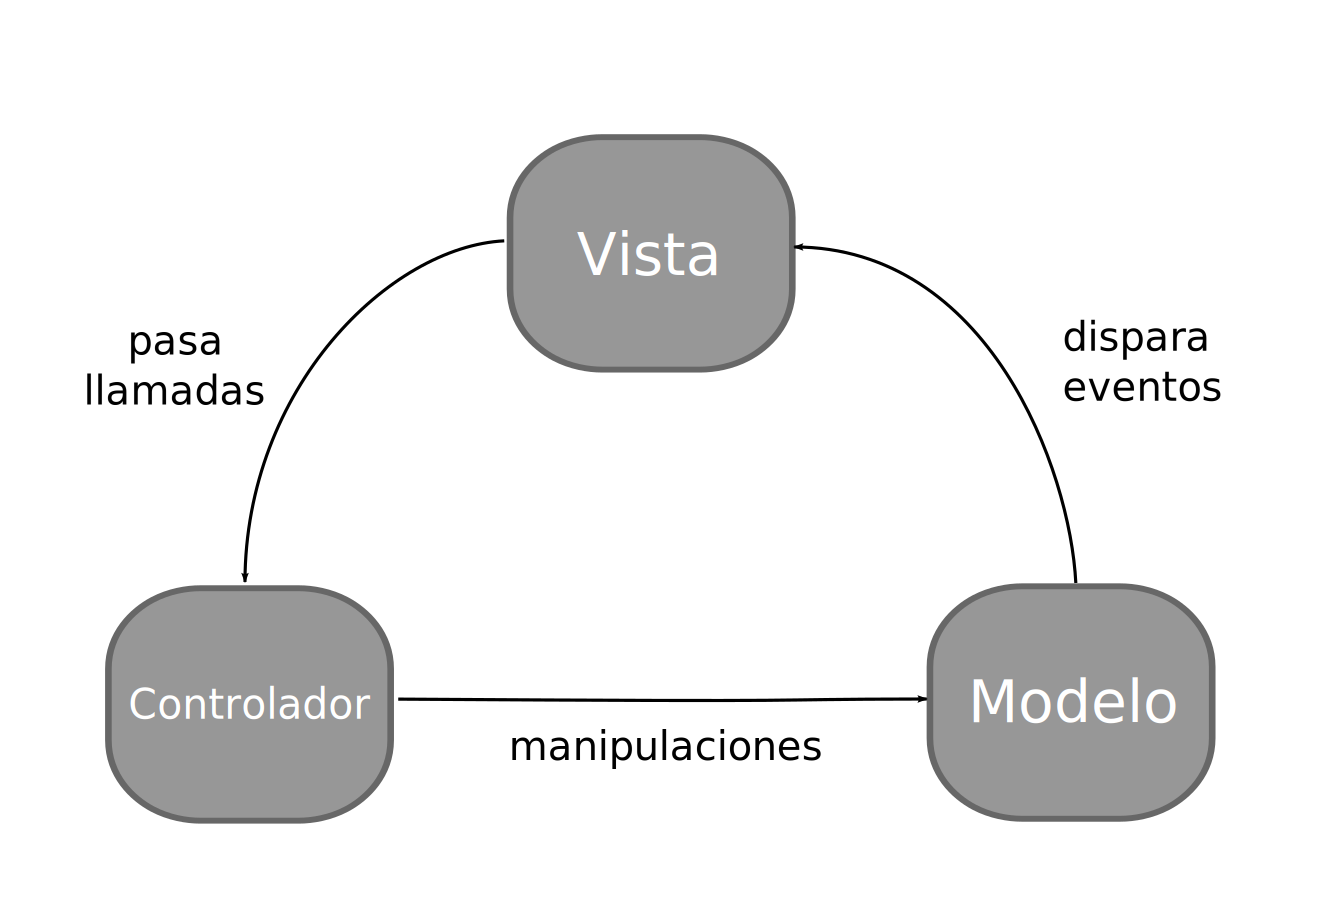
\includegraphics[width=250px]{src/img/MVC-vectorized.pdf}
        \caption[Interacción MVC] {Interacción MVC}
        \label{fig:InteraccionMVC}
    \end{center}
\end{figure}

El modelo es la especificación XML o \acs{DTD}\label{acro:DTD} (almacena la
información y describe su formato), que posteriormente es analizado y validado
en el controlador para constituir un modelo correcto y que sirve como componente 
intermedio para la comunicación y la gestión 
de los datos. Normalmente el formato del modelo sigue algún estándar definido
por alguna organización como la \acs{W3C}\label{acro:W3C},
\acs{IEEE}\label{acro:IEEE} o similares.

El análisis y validación puede realizarse en varias fases. Por ejemplo para 
omitir tipos de datos no requeridos o complejos. Una vez finalizado es expuesto
o renderizado en la vista que realiza una representación gráfica de 
la información.

En esta sección hemos comprobado como la generación dinámica de interfaces
son una opción más eficiente en aplicaciones donde no existen necesidades
estáticas. En la siguiente sección estudiaremos un caso de estudio que
modificará la interfaz para aprovechar las características de un buen
diseño.

\section{\uppercase{Caso de Estudio de American Airlines}}

En 2007 la compañía de aerolíneas ``American Airlines'' decidió realizar un
completo estudio\cite{Hud10} y rediseño de sus kioscos de compra de billetes y
check-in.

La aplicación anterior no resultaba completamente efectiva. Se ejecutaba sobre
un kiosco con una pantalla interactiva donde los pasajeros confirmaban su
llegada con número de ticket, comprobaban el estado de sus equipajes, etc.

\newpage

Su diseño inicial nunca tuvo en mente características como: el flujo real del
proceso que necesitaba la aplicación o patrones de diseño involucrados. El 
objetivo fue realizar una interfaz más consistente, fácil de traducir y 
más usable y amigable para los pasajeros de American Airlines.

\subsection{\uppercase{Mensajes y traducciones}}

En la primera etapa, se abordó rediseñar la interfaz teniendo en cuenta
la internacionalización. Durante la internacionalización del proyecto se idearon textos
instruccionales e indicativos en la parte superior de la pantalla. La usabilidad
fue probada en varias iteraciones en una atmósfera real como un aeropuerto.

Reducir la cantidad de texto y su complejidad en el diseño ayudo a la traducción
sencilla a otros idiomas. Los pasajeros demostraron una mayor interacción con la
interfaz y durante un tiempo menor. De forma adicional, para idiomas específicos
se añadieron textos en contexto para el idioma nativo que permitían aclarar
elementos especiales.

\subsection{\uppercase{Pantalla de inicio}}

En la segunda etapa, se valoró realizar un diseño de la pantalla de inicio. La
pantalla de inicio presentaba inconsistencias en el tamaño de los botones y
representación de iconos.

\begin{figure}[ht]
    \begin{center}
        \includegraphics[width=425px]{src/img/american-airlines-welcome-screen.pdf}
        \caption[American Airlines: Pantalla de
        bienvenida original (a) y mejorada (b)] {American Airlines: Pantalla de
        bienvenida original (a) y mejorada (b)}
        \label{fig:AmericanWelcome}
    \end{center}
\end{figure}

\newpage

Su agrupación no seguía un foco lógico para el usuario identificándolos con
botones extraños o poco utilizables. Esto confundía especialmente a nuevos
usuarios de la aplicación que desconocían complementamente su funcionamiento.

Otro cambio en este apartado fue el cambio de un diseño con fondo de
elementos distractorios a uno simplificado en tonos suaves y uniformes para
toda la aplicación.

En la figura ~\ref{fig:AmericanWelcome} se puede apreciar el cambio entre la
pantalla de inicio original y su posterior rediseño con una interfaz más
definida.

\subsection{\uppercase{Comprobación de equipajes}}

\begin{figure}[ht]
    \begin{center}
        \includegraphics[width=425px]{src/img/american-baggages.pdf}
        \caption[Pantalla de
        equipajes original (superior izquierda) y división en mejoradas (resto)]
        {Pantalla de
        equipajes original (superior izquierda) y división en mejoradas (resto)}
        \label{fig:AmericanBaggages}
    \end{center}
\end{figure}

\newpage

Durante la flexibilización del rediseño, se experimento con varias mejoras en el
campo de usabilidad en la sección de comprobación de equipajes. La pantalla
original contenía tres puntos separados de decisión. 

Las buenas prácticas de 
desarrollo de interfaces recomiendan no introducir elementos 
ambiguos en las decisiones de una pantalla. Por tanto se eliminó la opción de
pagos y se modificó de forma consistente con otras pantallas de pago.

La sección de dispositivos de ayuda se construyo con un mensaje (popup)
emergente accionado sólo por un criterio específico que definió las reglas de la
compañía. Para las transacciones monetarias se cambio al color verde en el
cuerpo de la pantalla.

\subsection{\uppercase{Opciones de itinerario}}

En el caso de los itinerarios de usuario la pantalla presentada era una de las
más complejas de la aplicación. En ella residía la mayoría de características
del kiosco interactivo.

Se eliminó el banner superior establecido de fondo en la pantalla en
consecuencia con lo establecido en la pantalla de inicio. El usuario se dirigió
a un itinerario de ventanas emergentes y de pantallas seguidas en consecuencia 
de las opciones elegidas. Aunque este cambio conllevó un mayor número de
pantallas y espacio, el usuario fácilmente identificaba cada característica 
con una nueva pantalla.
 
La sección de opciones del lado derecho, tenían unos colores en
consistencia al resto de la aplicación. En el estado de selección los botones
fueron oscurecidos. Se añadió una barra de desplazamiento para que todos los
elementos pudieran encajar en la pantalla mediante deslizamiento. En el 
pasado era necesario cambiar entre pantallas para ver el contenido.

\begin{figure}[ht]
    \begin{center}
        \includegraphics[width=425px]{src/img/american-itinerary.pdf}
        \caption[Opciones de itinerario original (a) y mejorado (b)] 
        {Opciones de itinerario original (a) y mejorado (b)}
        \label{fig:AmericanItinerary}
    \end{center}
\end{figure}

Con el soporte del cliente interno y la retroalimentación del departamento de IT
la compañia American Airlines consiguió una grandiosa mejora en el aspecto de
usabilidad del kiosco interactivo, mejora de consistencia, incremento de
espacios en blanco, robustez, internacionalización con múltiples idiomas, reducción
del número de clicks para realizar tareas y ajuste del flujo de la aplicación.

En conclusión, el estudio meditado de una interfaz es una tarea significante el
el desarrollo de una aplicación. En FreeStation se ha facilitado la construcción
y adaptación de interfaces dinámicamente, de modo que la vista ofrecida al
usuario pueda ser fácilmente modificada, minimizando los enormes costes
relativos a la adaptación de interfaces en POIs.
%% Put a blank page for open next chapter on right page side
%%\newpage
%\mbox{}
%\thispagestyle{empty}